\section{System Evaluation}
\label{chap:5}

In this section, the system evaluation is explained in details. The randomised distributed algorithm proposed in \cite{yves2009optimal} was tested with three synchronization techniques explained in section \ref{chap:3} using the simulator described previously in section \ref{chap:4}. The model for generating random graph for the networks topologies are described in this section. The evaluation metrics, hardware and software used for testing and the simulation workflow are also part of this section.  

% The theoretical bound for this algorithm is known to be $O(\log N)$. The synchronizers time and message complexity were discussed in section \ref{chap:3}. 

\subsection{Evaluation Criteria}



The metrics used to measure the algorithm are time and  messages complexity. Time complexity  in the synchronous model is measure by counting the number of rounds until the algorithm terminates. Message complexity consists in counting the total number of messages send by the processes.

The aim of the simulation is to evaluate the time and messages complexity of the algorithm. Additionally, show how the synchronization techniques generate overhead over the synchronous algorithm and present a discussion about the trade off between the techniques based on experimental results.


\subsection{Network Models}
\label{sec:topology}


The network topologies need to be generated before testing the \textit{MIS} algorithm. Topologies represent the distributed system in which the algorithm is going to be tested. Processors are mapped to vertices and the communication channels to edges.  The random graph model used to generate the networks topologies is call Stochastic Block Model \textbf{SBM}, proposed in \cite{holland1983stochastic}.

Before entering in details on the SBM, a brief explanation about the Erd\~os--R\'enyi model is presented. This model is used to generate random graphs and it was first proposed in \cite{erdds1959random}. There are two variants of this model, one of them is the $G(n, p)$ model in which a graph is constructed by connecting $n$ vertices randomly. An edge is included in the graph between two vertices $i,j$ with independent probability $p$. On \cite{erdos1960evolution} Erd\~os and R\'enyi presented some important properties about random graph. These properties about connectivity are used to generate the topologies for the simulations of this project and are cited below.


\begin{enumerate}
\item If $p<{\tfrac {(1-\epsilon )\ln n}{n}}$, then the graph $G(n, p)$ it is very likely to be disconnected.
\item If $p>{\tfrac {(1+\epsilon )\ln n}{n}}$ , then the graph $G(n, p)$ it is very likely to be connected.
\end{enumerate}

The key conclusion is that if connected graphs are needed, then ${\tfrac {\ln n}{n}}$ is the threshold of $p$ for which the generated graphs $G(n, p)$ will almost surely be connected.  

In the SBM, the networks are characterised by blocks structures, these blocks define partitions of the networks. Every vertex is associated with a group and the distribution of the edges between vertices depend on the group in which a vertex is member. It is possible to obtain graphs that are denser in some regions playing with the probabilities of the groups or blocks. The probability for each group is defined in a probability matrix. In the next section, a formal definition of the \textit{SBM} is given with some examples of graphs generated by this model.


\subsection{Stochastic Block Model}

The SBM can be considered a probabilistic or generative model in which a probability is assigned to each pair of vertices $i,j$ in the network. This model defines a probability distribution over networks $Pr(G | \theta)$, where $\theta$ is a set of parameters that define the graph. For a given $\theta$, it is possible to generate a network instance G by flipping a coin between every possible pair of vertices of the $G$ according to the probability distribution.  

The Stochastic Block Model is formally defined by: 
\begin{enumerate}

    \item $k$: a scalar representing the number of blocks groups, clusters or modules in the network.
    \item $\overrightarrow{z}$: a vector of n element where $z(l)$ gives the block index of the vertex $l$.
    \item $M$ is a $k * k$ stochastic block matrix, where $M_{ij}$ gives the probability that a vertex of block type $i$ is connected to a vertex of block type $j$.
\end{enumerate}


The edges generated by flipping the coin between each pair of vertices have probability independence but are not necessarily identically distributed. A large number of parameters allows the SBM  to produce very different structures. If $M_{ij} = p$ for each pair of blocks, then the SBM is reduced to the Erd\~os--R\'enyi model of random graph $G(n,p)$. The figure \ref{fig:erdos} show an example of stochastic block matrix in which every probability is the same for $k = 3$ blocks. Note that this is a square matrix and $k$ should be defined before $z$ and $M$. It can be seen that the probability distribution is the same for each block, as a consequence, the graph looks like one component even if the vertex belongs to different blocks types.

 In the figure \ref{fig:sbm}, another example of a random graph is shown, however, in this example the probability distribution differ between blocks and it is more easy to visualize the different groups in the picture. The entrance $M_{i,j}$ where $i = j$ represent the probability of one edge between two vertices in the same group and the entrance $M_{i,j}$ where $i \neq j$ represent the probability of one edge between two vertices in the different groups. 

When $M_{i,i}$ is greater than $M_{i,j}$ for $i \neq j$ the vertices tend to connect other vertices that are in the same group. For this configuration the values of the diagonal are larger than values off it, in this case, it is the communities are assortative and the edges are more common within the blocks. On the contrary, on disassortative communities, edges between vertex of different communities are more common $M_{ii} <  M_{ij}$ for $i \neq j$.


Many other grouping criteria and variation of \textit{SBM} exist in the literature \cite{carrington2005models,holland1983stochastic,airoldi2008mixed}. Particularly, for this project, the assortative grouping is used for generating topologies. The ${\tfrac {\ln n}{n}}$ threshold is used to set the probability of the diagonal in the block matrix of probabilities. 





\begin{figure}[ht]
\centering
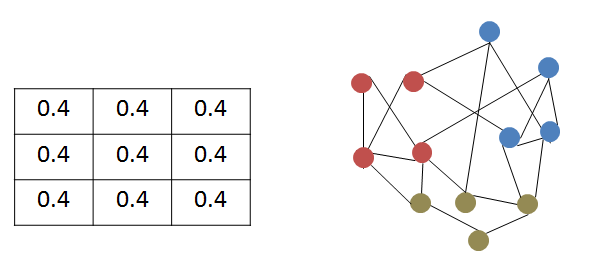
\includegraphics[width=1 \linewidth, height=5cm]{Erdos-Renyi.PNG} 
\caption{Example of SBM with equal probabilities}
\label{fig:erdos}
\end{figure}

\begin{figure}[ht]
\centering
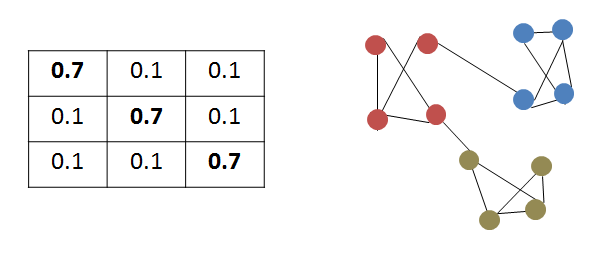
\includegraphics[width=1 \linewidth, height=5cm]{sbm.PNG} 
\caption{Example of SBM with assortative communities}
\label{fig:sbm}
\end{figure}

\subsection{Description of Experiments}

As mention in section \ref{chap:4}, the simulator was implemented in Elixir 1.6. The topology generator used to create network topology is an open source software written in Python under MIT license. Some modifications were done to the generator, for instance, compute the probability only for the upper triangular adjacency matrix of the topology, modified the parameters, customised the file format for store the topologies and some other minors modifications. 

The tests were run in a computer with processor Intel(R) Core(TM) i5--4210U of 1.7 and 2.4 GHz and RAM memory of 8 GB with additional 8 GB of SWAP. The operating system was a Linux 64 bit Debian base.


The value for $p$ was chosen to make sure that the generated graph is connected for the \textit{SBM}. Note that the algorithm for \textit{MIS} does not require this condition because it still finds the solution for a disconnected graph. However, the Beta Synchronizer construct a rooted spanning tree over the topology in order to send \textbf{safe} and \textbf{go} messages to the root and from it, so if the topology is not connected the rooted spanning tree can not be constructed. In order to maintain the same topologies for every simulation, the generated graphs are always connected.  

The steps to perform the experiments are enumerated below:

\begin{enumerate}
\item Implementation of the synchronizers Alpha and Beta.
\item Implementation of the Maximal Independent Set algorithm using the simulation developed in step 1.
\item Implementation of the Maximal Independent Set Algorithm using a global synchronization technique.
\item Create the topology with the Stochastic Block Model according to the description in the section \ref{sec:topology}.
\item Run N times the synchronous algorithm for the \textit{MIS} and saves the results for each synchronizer technique (Alpha, Beta and Global).
\item Compute the average and calculate the results.
\end{enumerate}



